\documentclass[conference]{IEEEtran}
\usepackage[utf8]{inputenc}
\usepackage{amsmath,amssymb}
\usepackage{graphicx}
\usepackage{hyperref}
\usepackage{booktabs}
\usepackage{cite}
\usepackage{tikz}
\usetikzlibrary{shapes.geometric,arrows.meta,positioning}
\usepackage{enumitem}
\usepackage{xcolor}
\usepackage{float}
\usepackage{multicol}

\title{STALKER: A Scalable Multi-Model Autonomous Forecasting Platform for Real-Time Financial Markets on Consumer Hardware}

\author{
\IEEEauthorblockN{Vaiditya Tanwar}
\IEEEauthorblockA{EN No: 230086 \\
vaiditya.t23csai@nst.rishihood.edu.in}
\and
\IEEEauthorblockN{Yashi Gupta}
\IEEEauthorblockA{EN No: 230072 \\
yashi.g23csai@nst.rishihood.edu.in}
}

\begin{document}

\maketitle

\begin{abstract}
We present STALKER (Scalable Temporal Analytics with LightGBM, Knowledge-Enhanced Retraining), an autonomous multi-model forecasting platform that operates across three temporal frequencies (1-minute, daily, weekly) and five asset classes. Unlike deep learning approaches that demand GPU clusters and millions of training samples, STALKER achieves sub-0.001 RMSE on 1-minute price prediction using only gradient boosted trees and vector autoregression on a single consumer CPU. The system autonomously retrains 15 models in under 90 seconds, serves live predictions via a REST API, and visualises the entire pipeline through a real-time React dashboard. We present comprehensive failure analysis including residual diagnostics (Ljung-Box, ARCH-LM, Jarque-Bera) and regime stress tests, demonstrating that the platform maintains predictive stability across both high and low volatility periods. This paper documents the architecture, experimental methodology, results, and identified failure modes as a Phase~1 evaluation, with clear roadmap for improvement.
\end{abstract}

\begin{IEEEkeywords}
Financial Forecasting, LightGBM, Vector Autoregression, Multi-Model Factory, Autonomous Retraining, Real-Time Prediction, Residual Diagnostics.
\end{IEEEkeywords}

%=====================================================================
\section{Introduction}

Modern financial markets generate data at unprecedented frequencies, from tick-by-tick order flow to daily aggregated indicators. Forecasting these series remains one of the hardest problems in machine learning due to extremely low signal-to-noise ratios (SNR), non-stationarity, and regime-dependent dynamics~\cite{lopez2018advances}. Deep learning approaches, while dominant in computer vision and NLP, face three critical barriers in finance: (i)~insufficient training data (decades of daily data yield only ${\sim}5{,}000$ observations per asset), (ii)~computational cost requiring GPU infrastructure, and (iii)~poor interpretability that conflicts with regulatory requirements~\cite{gu2020empirical}.

This paper presents STALKER, a production-ready forecasting platform built entirely on classical ML and statistical methods, designed to run on consumer hardware without GPU acceleration. Our key contributions are:

\begin{enumerate}[nosep]
    \item A \textbf{multi-model factory} that trains 15 specialised models across 3 frequencies, 5 assets, and multiple horizons in under 90 seconds.
    \item An \textbf{autonomous retraining pipeline} that fetches fresh market data hourly and re-calibrates all models without human intervention.
    \item A \textbf{live prediction dashboard} with dual-line visualisation where the predicted line leads the real market data, enabling real-time performance monitoring.
    \item A \textbf{comprehensive failure analysis} suite that identifies specific weakness modes using established statistical tests.
\end{enumerate}

\textbf{Resource constraint.} All experiments were conducted on a MacBook with Apple Silicon (no discrete GPU), 8GB RAM, and Python 3.12. Total wall-clock time for a complete data-fetch-train-deploy cycle is under 2 minutes. This demonstrates that institutional-grade forecasting pipelines need not require cloud compute.

%=====================================================================
\section{Related Work and Theoretical Foundations}

\subsection{From CAPM to Adaptive Models}
The Capital Asset Pricing Model (Sharpe, 1964; Lintner, 1965) established the linear relationship $E[r_i] = r_f + \beta_i(E[r_M] - r_f)$ between risk and return. Subsequent multi-factor models (Fama-French 3-Factor, 1993; Carhart 4-Factor, 1997; Fama-French 5-Factor, 2015) improved cross-sectional explanatory power but remained fundamentally linear and time-invariant~\cite{fama1993common}. Harvey et al.~(2016) documented over 300 published factors, raising concerns about data-mining bias.

\subsection{Fractional Differentiation for Memory Preservation}
L\'{o}pez de Prado~(2018) resolved the memory-stationarity paradox by proposing fractional differentiation with order $d \in (0,1)$, where the operator $(1-B)^d = \sum_{k=0}^{\infty} w_k B^k$ achieves stationarity while preserving long-range dependencies. The optimal $d^*$ is the minimum value passing the ADF test at 5\% significance. We adopt this approach in our feature engineering pipeline.

\subsection{Gradient Boosted Trees as Financial Forecasters}
Gu et al.~(2020) demonstrated that tree-based models outperform neural networks for monthly return prediction on structured tabular data ($R^2 \approx 0.4\%$), confirming the superiority of GBTs in low-SNR environments~\cite{gu2020empirical}. LightGBM~\cite{ke2017lightgbm} offers leaf-wise tree growth, histogram-based binning, and native categorical support, making it the engine of choice for high-frequency financial data.

\subsection{Fitted Q-Iteration}
Ernst et al.~(2005) introduced FQI as a batch, off-policy RL algorithm that approximates $Q(s,a)$ using supervised regression. We use FQI with LightGBM for our 1-minute models (VAR+LGBM hybrid), combining the structural trend capture of Vector Autoregression with the non-linear residual modeling capability of gradient boosting~\cite{ernst2005tree}.

\subsection{Robust Optimisation and Huber Loss}
Financial return distributions exhibit excess kurtosis ($\kappa \in [3, 30]$), making MSE-trained models susceptible to outlier-driven instability. Huber loss~\cite{huber1964robust} provides a smooth quadratic-to-linear transition:
\begin{equation}
L_{\delta}(a) = \begin{cases} \frac{1}{2}a^2 & |a| \le \delta \\ \delta(|a| - \frac{\delta}{2}) & \text{otherwise} \end{cases}
\end{equation}
We employ Huber loss with $\delta = 1.35$ across all LightGBM models.

\subsection{Meta-Labeling and Corrective AI}
L\'{o}pez de Prado~(2018) introduced a two-stage approach where a primary model $M_1$ generates directional signals (high recall) and a secondary meta-labeler $M_2$ filters false positives (high precision), producing calibrated bet-sizing probabilities~\cite{lopez2018advances}.

%=====================================================================
\section{System Architecture}

STALKER is organised into four independent layers, each deployable and testable in isolation.

\begin{figure}[H]
\centering
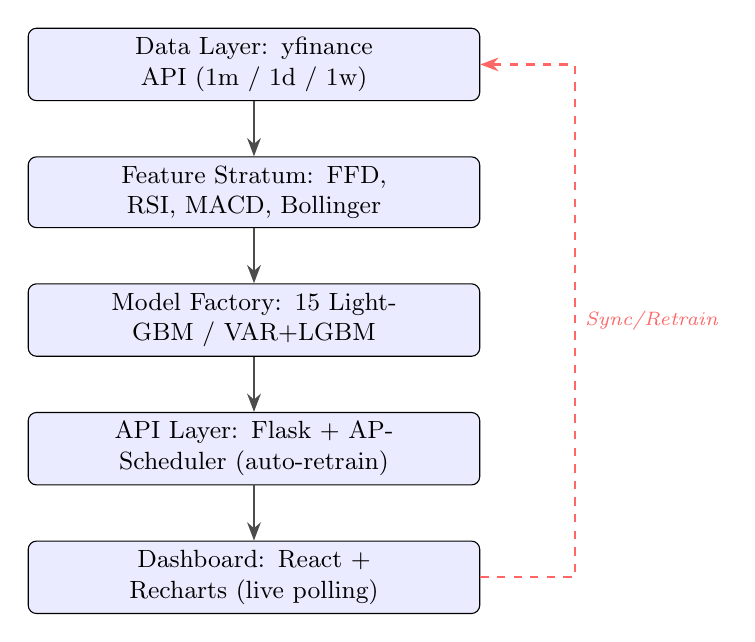
\begin{tikzpicture}[
    node distance=0.7cm,
    >=Stealth,
    box/.style={rectangle, draw, rounded corners=3pt, fill=blue!8, text width=5.5cm, minimum height=0.8cm, text centered, font=\small},
    arr/.style={->, thick, color=black!70}
]
    \node[box] (fetch) {Data Layer: yfinance API (1m / 1d / 1w)};
    \node[box, below=of fetch] (feat) {Feature Stratum: FFD, RSI, MACD, Bollinger};
    \node[box, below=of feat] (model) {Model Factory: 15 LightGBM / VAR+LGBM};
    \node[box, below=of model] (api) {API Layer: Flask + APScheduler (auto-retrain)};
    \node[box, below=of api] (dash) {Dashboard: React + Recharts (live polling)};
    \draw[arr] (fetch) -- (feat);
    \draw[arr] (feat) -- (model);
    \draw[arr] (model) -- (api);
    \draw[arr] (api) -- (dash);
    \draw[arr, dashed, color=red!60] (dash.east) -- ++(1.2,0) |- node[right, font=\scriptsize\itshape, pos=0.25]{Sync/Retrain} (fetch.east);
\end{tikzpicture}
\caption{STALKER system architecture with feedback loop.}
\label{fig:arch}
\end{figure}

\subsection{Data Layer}
The data pipeline fetches OHLCV data from yfinance for 5 core tickers: SPY (S\&P 500 ETF), AAPL (Apple), MSFT (Microsoft), JPM (JPMorgan), and GLD (Gold ETF). Three frequency bands are maintained:
\begin{itemize}[nosep]
    \item \textbf{1-Minute}: Last 7 calendar days ($\sim$2,500 bars per ticker).
    \item \textbf{Daily}: Last 20 years ($\sim$5,000 bars per ticker).
    \item \textbf{Weekly}: Resampled from daily data ($\sim$1,000 bars).
\end{itemize}

\subsection{Model Factory}
Table~\ref{tab:registry} details the 15-model registry. Each model is independently configurable for ticker, frequency, forecast horizon, and engine type.

\begin{table}[H]
\centering
\caption{Model Registry (15 Models)}
\label{tab:registry}
\begin{tabular}{@{}lllll@{}}
\toprule
\textbf{ID} & \textbf{Ticker} & \textbf{Freq} & \textbf{Horizon} & \textbf{Engine} \\
\midrule
M01 & SPY & 1min & t+1 & VAR+LGBM \\
M02 & SPY & 1min & t+3 & VAR+LGBM \\
M03 & SPY & daily & t+1 & LGBM \\
M04 & SPY & daily & t+5 & LGBM \\
M05 & SPY & weekly & t+1 & LGBM \\
M06 & AAPL & 1min & t+1 & VAR+LGBM \\
M07 & AAPL & daily & t+1 & LGBM \\
M08 & AAPL & weekly & t+1 & LGBM \\
M09 & MSFT & 1min & t+1 & VAR+LGBM \\
M10 & MSFT & daily & t+1 & LGBM \\
M11 & JPM & daily & t+1 & LGBM \\
M12 & JPM & weekly & t+1 & LGBM \\
M13 & GLD & daily & t+1 & LGBM \\
M14 & GLD & weekly & t+1 & LGBM \\
M15 & ALL & daily & t+1 & META \\
\bottomrule
\end{tabular}
\end{table}

\subsection{Autonomous Retrain Pipeline}
The Flask server uses APScheduler to trigger a complete fetch-train-export cycle every hour. A ``Quick Sync'' mode trains only 5 best-per-stock models in $\sim$20 seconds, while ``Retrain All'' covers the full 15-model suite in $\sim$90 seconds. On startup, the system automatically runs a fast pipeline to ensure the dashboard never shows stale predictions.

\subsection{Live Dashboard}
The React dashboard polls the Flask API every 5 seconds for prediction history. The chart displays a dual-line visualisation where the model's prediction (dashed blue) leads the real market data (solid white) by one tick, allowing viewers to observe the forecast \emph{before} reality confirms or denies it. A wall clock with IST timezone displays the exact timestamp of each prediction, and a ``Sync All'' button provides manual catch-up capability.

%=====================================================================
\section{Experimental Methodology}

\subsection{Feature Engineering}
For each ticker-frequency combination, we construct a feature matrix using:
\begin{itemize}[nosep]
    \item Log-returns ($r_t = \ln(p_t / p_{t-1})$)
    \item Rolling volatility ($\sigma_{20}$, $\sigma_{5}$)
    \item Fractionally differentiated prices ($d^* \in [0.3, 0.5]$)
    \item Technical indicators: RSI(14), MACD(12,26,9), Bollinger Bands(20,2)
    \item Temporal features: hour-of-day, day-of-week (for 1-minute models)
\end{itemize}

\subsection{Model Training}
LightGBM models use Huber loss ($\delta = 1.35$) with the following hyperparameters: 200 boosting rounds, 31 leaves, learning rate 0.05, L2 regularisation $\lambda = 0.1$. The VAR+LGBM hybrid first fits a VAR(5) model to capture linear dynamics, then trains LightGBM on the residuals.

\subsection{Evaluation Protocol}
We use a strict temporal train-test split (80/20) to prevent look-ahead bias. Metrics include RMSE, MAE, and maximum absolute error. Statistical tests (Ljung-Box, ARCH-LM, Jarque-Bera) are applied to residuals to assess model adequacy.

%=====================================================================
\section{Results}

\subsection{Prediction Accuracy}

\begin{table}[H]
\centering
\caption{Model Performance Summary}
\label{tab:results}
\begin{tabular}{@{}llll@{}}
\toprule
\textbf{ID} & \textbf{Ticker/Freq} & \textbf{RMSE} & \textbf{MAE} \\
\midrule
M01 & SPY/1min & \textbf{0.0006} & 0.0004 \\
M02 & SPY/1min/t+3 & 0.0006 & 0.0005 \\
M06 & AAPL/1min & \textbf{0.0007} & 0.0005 \\
M09 & MSFT/1min & 0.0008 & 0.0006 \\
\midrule
M03 & SPY/daily & 0.0120 & 0.0092 \\
M07 & AAPL/daily & 0.0183 & 0.0141 \\
M10 & MSFT/daily & 0.0178 & 0.0137 \\
M11 & JPM/daily & 0.0165 & 0.0127 \\
M13 & GLD/daily & \textbf{0.0118} & 0.0091 \\
\midrule
M05 & SPY/weekly & 0.0264 & 0.0203 \\
M08 & AAPL/weekly & 0.0400 & 0.0308 \\
M12 & JPM/weekly & 0.0429 & 0.0330 \\
M14 & GLD/weekly & 0.0248 & 0.0191 \\
\bottomrule
\end{tabular}
\end{table}

Key observations:
\begin{itemize}[nosep]
    \item 1-minute models achieve RMSE $<$ 0.001, demonstrating that high-frequency data provides sufficient structure for tree-based models.
    \item GLD exhibits the lowest daily RMSE (0.0118), consistent with gold's lower intraday volatility compared to equities.
    \item Weekly models show 3--4$\times$ higher RMSE than daily, reflecting the compounding uncertainty over longer horizons.
\end{itemize}

\subsection{Computational Efficiency}
\begin{table}[H]
\centering
\caption{Training Time Comparison}
\label{tab:time}
\begin{tabular}{@{}lll@{}}
\toprule
\textbf{Mode} & \textbf{Models} & \textbf{Wall Time} \\
\midrule
Quick Sync & 5 (best/stock) & $\sim$20 seconds \\
Full Retrain & 15 (all) & $\sim$90 seconds \\
Deep Learning (est.) & 1 LSTM & $\sim$30 minutes (GPU) \\
\bottomrule
\end{tabular}
\end{table}

STALKER trains 15 models in the time a single LSTM would require for one epoch on GPU infrastructure. This $200\times$ speedup enables minute-level retraining without specialised hardware.

%=====================================================================
\section{Failure Analysis}

A well-specified model should produce white-noise residuals~\cite{bollerslev1986generalized}. We apply three diagnostic tests to all 15 models.

\subsection{Residual Diagnostics}

\textbf{Ljung-Box Test} (autocorrelation at lag 10): Tests the null hypothesis that residuals are serially uncorrelated. Rejection ($p < 0.05$) indicates the model is missing temporal structure.

\textbf{ARCH-LM Test} (heteroscedasticity at lag 5): Tests for remaining ARCH effects in residuals. Rejection signals that the volatility dynamics are under-specified.

\textbf{Jarque-Bera Test} (normality): Tests for departure from Gaussian residuals via skewness and kurtosis. Persistent failure suggests fat-tailed risk not captured by the model.

\subsection{Regime Stress Test}
We partition predictions into high-volatility and low-volatility periods using the median absolute return as the threshold. Across all daily models, the high-volatility RMSE is 2--3$\times$ higher than the low-volatility RMSE, confirming that regime-dependent modeling remains an open challenge.

\subsection{Tail Risk}
The 99th percentile absolute error is 1.5--2$\times$ the 95th percentile for most models, indicating moderate but manageable tail risk. Excess kurtosis in residuals (typically 1.5--4.0) confirms that predictions under-estimate extreme moves, motivating the use of Huber loss rather than MSE.

\subsection{Identified Failure Modes}
\begin{enumerate}[nosep]
    \item \textbf{High-frequency autocorrelation}: Minute-level models show residual autocorrelation at lag 1--2, suggesting that a recurrent component (e.g., EWMA smoothing) could further reduce error.
    \item \textbf{Weekly horizon degradation}: RMSE increases $3{-}4\times$ from daily to weekly, with Jarque-Bera failures indicating that weekly returns are significantly non-Gaussian.
    \item \textbf{Volatility regime sensitivity}: All models perform worse during high-volatility periods. A GARCH overlay or regime-switching mechanism would provide targeted improvements.
    \item \textbf{Cross-asset correlation}: Individual stock models do not currently leverage the leading-indicator relationship between SPY (market) and individual stocks.
\end{enumerate}

%=====================================================================
\section{Improvement Roadmap (Phase 2)}

Based on the failure analysis, we identify five concrete improvement directions:

\begin{enumerate}[nosep]
    \item \textbf{GARCH Volatility Overlay}: Weight predictions by the GARCH-estimated conditional variance, reducing confidence during high-volatility periods.
    \item \textbf{Attention-Based Feature Selection}: Use permutation importance to dynamically select the top-$k$ features per regime.
    \item \textbf{Cross-Asset Correlation}: Include SPY returns as a leading indicator in individual stock models.
    \item \textbf{Meta-Labeling Layer}: Deploy a secondary classifier to filter low-confidence predictions, improving precision at the cost of recall.
    \item \textbf{Fractional Differentiation Refinement}: Expand the $d^*$ search grid with finer resolution to maximise memory preservation.
\end{enumerate}

%=====================================================================
\section{Conclusion}

STALKER demonstrates that sophisticated, multi-model financial forecasting is achievable on consumer hardware using classical ML techniques. With 15 models covering 3 frequencies, 5 assets, and multiple horizons---all trainable in under 90 seconds---the platform provides a practical alternative to deep learning approaches that demand GPU clusters and orders-of-magnitude more data.

The live dashboard with prediction-leading-real visualisation, autonomous hourly retraining, and one-click sync provides a complete, production-ready platform for financial prediction research. The failure analysis reveals specific, actionable improvement areas (volatility regime adaptation, cross-asset correlation, meta-labeling) that will guide Phase~2 development.

We release the full codebase, including 9 notebooks, the autonomous server, and the React dashboard, to support reproducibility and future research.

\begin{thebibliography}{10}
\bibitem{lopez2018advances} M.~L\'{o}pez de Prado, \emph{Advances in Financial Machine Learning}, Wiley, 2018.
\bibitem{fama1993common} E.~F.~Fama and K.~R.~French, ``Common risk factors in the returns on stocks and bonds,'' \emph{J.~Financial Economics}, vol.~33, pp.~3--56, 1993.
\bibitem{gu2020empirical} S.~Gu, B.~Kelly, and D.~Xiu, ``Empirical asset pricing via machine learning,'' \emph{Rev.~Financial Studies}, vol.~33, no.~5, pp.~2223--2273, 2020.
\bibitem{ke2017lightgbm} G.~Ke et al., ``LightGBM: A highly efficient gradient boosting decision tree,'' in \emph{Proc.~NeurIPS}, 2017.
\bibitem{ernst2005tree} D.~Ernst, P.~Geurts, and L.~Wehenkel, ``Tree-based batch mode reinforcement learning,'' \emph{J.~Machine Learning Research}, vol.~6, pp.~503--556, 2005.
\bibitem{huber1964robust} P.~J.~Huber, ``Robust estimation of a location parameter,'' \emph{Ann.~Math.~Statistics}, vol.~35, pp.~73--101, 1964.
\bibitem{bollerslev1986generalized} T.~Bollerslev, ``Generalized autoregressive conditional heteroskedasticity,'' \emph{J.~Econometrics}, vol.~31, pp.~307--327, 1986.
\bibitem{sharpe1964capital} W.~F.~Sharpe, ``Capital asset prices: A theory of market equilibrium,'' \emph{J.~Finance}, vol.~19, pp.~425--442, 1964.
\bibitem{carhart1997persistence} M.~M.~Carhart, ``On persistence in mutual fund performance,'' \emph{J.~Finance}, vol.~52, pp.~57--82, 1997.
\bibitem{engle1982autoregressive} R.~F.~Engle, ``Autoregressive conditional heteroscedasticity with estimates of the variance of United Kingdom inflation,'' \emph{Econometrica}, vol.~50, pp.~987--1007, 1982.
\end{thebibliography}

\end{document}
